\section{Problem Definition}
\label{sec:problem_definition}
%\todo[author=DSN,inline]{Can we refrain from referring to Challenges and attacks as 'Challenge 1-2-3', 'Attack 1-2-3'? We can give abbreviations to them and use the abbreviations throughout the paper. Otherwise it is hard for the reader to remember what 1-2-3 stands for.}
%\todo[author=SB,inline]{Changed the numberings to names, please check!}
%\noindent Researchers in ~\cite{cloud-malware:2016}, \cite{automated-detection:2016}, \cite{UBL:2012} attempt to address \textit{challenge 1} by proposing unsupervised and semi-supervised machine learning algorithms such as K-Means, Self Organising Map (SOM) algorithms, and one class Support Vector Machine (SVM). 
%They also use averaging on the raw data as a data pre-processing step to address \textit{challenge 2}.
%Researchers in~\cite{EbAT:2010}, \cite{entorpy_based_detection_2:2014}, \cite{density-based:2016} consider data distribution (entropy and density) to solve \textit{challenge 1} and \textit{challenge 2}.
%They also use averaging on the raw data as a data pre-processing step to address \textit{challenge 2}. Researchers in~\cite{EbAT:2010} and \cite{entorpy_based_detection_1:2005} consider data distribution (entropy and density) to solve \textit{challenge 1} and \textit{challenge 2}. 
%Although these approaches help intrusion detection systems (IDSs) to achieve high accuracy with low false positive rates, they may suffer from accuracy and false alarm issues in certain scenarios for certain use cases.  
%To demonstrate this, 
%In order to showcase how state-of-the-art anomaly-based IDSs for Cloud may encounter accuracy and false alarm issues, we created a scenario where a Cloud application runs in one of the VMs in a Cloud data centre and at one stage the application suffers from a backdoor channel attack that increases its resource utilisation, specifically, the CPU utilisation. We built the Cloud data centre in our lab using OpenStack\footnote{https://www.openstack.org} (details of the set-up are available in Section~\ref{sec:experiments}) and executed one Graph Analytics workload (collected from CloudSuite\footnote{http://cloudsuite.ch}) as the Cloud application in one of the VMs hosted in our lab-based Cloud data centre. 
%In this section we showcase how the state-of-the-art average~\cite{automated-detection:2016}, \cite{UBL:2012}, \cite{cloud-malware:2016}, and entropy~\cite{EbAT:2010}, \cite{entorpy_based_detection_2:2014} based data analysis may result in low accuracy and high false positive rate for anomaly detection systems in the Cloud.  In addition, we show how standard deviation based analysis may also raise accuracy and false positive issues.
%In this section we give a brief summary on how anomaly detection systems generally work in detecting cybersecurity attacks in the Cloud. Then, we highlight the underlying assumptions of such Cloud anomaly detection systems and define their key problems.  
%In this section we give a brief summary on how anomaly detection systems generally work in detecting cybersecurity attacks in the Cloud. Then, we define the key problems with these systems. 
\noindent In order to detect cybersecurity attacks in a Cloud data centre, anomaly detection systems generally make the following assumptions:
\begin{itemize} %[{(1)}] 
\item \textbf{Assumption-1:} Resource utilisation of a VM follows some kind of ``normal” behaviour or trend which can be modelled by using machine learning or statistical approaches.
\item \textbf{Assumption-2:} Cybersecurity attacks such as DDoS and crytomining attacks consume VM resources significantly. This results in a deviation in the ``normal” trend of a VM's resource utilisation, which can be captured as anomalous by the machine learning or statistical approaches.
%which can be captured as anomaly by the machine learning or statistical approaches. 
\end{itemize} %[{(1)}] 

Assumption-1 is very general and is considered by many anomaly detection systems like~\cite{automated-detection:2016}, \cite{UBL:2012}, \cite{cloud-malware:2016}, \cite{EbAT:2010}. 
%Assumption-2 is also considered by researchers in [] specifically for DDoS attacks. We find evidence of the impact of cryptomining attacks on CPU in these [REF] related work.  
Assumption-2 is experimentally demonstrated by~\cite{ddso_charater_2017} while they analysed real DDoS attack samples taken from the CAIDA\footnote{http://www.caida.org/data/passive/ddos-20070804\_dataset.xml} dataset. 
%A recent report\footnote{https://www.prnewswire.com/news-releases/radiflow-reveals-first-documented-cryptocurrency-malware-attack-on-a-scada-network-300595714.html} published by PR Newswire announces that 
%A recent report\footnote{https://www.prnewswire.com/news-releases/radiflow-reveals-first-documented-cryptocurrency-malware-attack-on-a-scada-network-300595714.html} announces that 
Recently, Radiflow\footnote{https://radiflow.com}, a cybersecurity solution provider, has discovered the first documented cryptomining attack on a SCADA network. According to Radiflow, cryptomining attacks cause high CPU and network bandwidth consumption. 
In our work, we also consider both these assumptions.
%Radiflow\footnote{https://radiflow.com} announces that has revealed the first documented cryptocurrency malware attack on a SCADA network of a critical infrastructure operator. that ,  We find evidence of the impact of cryptomining attacks on CPU in these [REF] related work.  

%\textcolor{red}{In most cases, the Cloud anomaly detection systems perform well under these assumptions, but, however, there are some cases where they may suffer from performance issues. We explain this in the following example: }
% how the state-of-the-art average~\cite{automated-detection:2016}, \cite{UBL:2012}, \cite{cloud-malware:2016}, and entropy~\cite{EbAT:2010}, \cite{entorpy_based_detection_2:2014} based data analysis may result in low accuracy and high false positive rate for anomaly detection systems in the Cloud.  In addition, we show how standard deviation based analysis may also raise accuracy and false positive issues.
%fail to differentiate genuine Cloud workload spikes from ``anomalous" behaviour and generate false positive whenever they encounter such spikes.  

In most cases, the Cloud anomaly detection systems perform well under these assumptions. However, there are some cases where they may suffer from performance issues. In this paper we specifically consider the case where a Cloud anomaly detection system is using a linear classifier like K-Means, SVM, Naive Bayes, etc., and the VMs are exhibiting workload spikes. We explain this in the following example.

\textit{Example Scenario:} We created an example scenario where a VM hosted in a Cloud data centre runs a Cloud application and at one stage the VM becomes compromised by a cryptomining attack that consumes its CPU to perform illicit cyrptocurrency mining. We built the Cloud data centre in our lab using OpenStack\footnote{https://www.openstack.org} (details of the set-up are available in Section~\ref{sec:experiments}) and executed a Graph Analytics workload (collected from CloudSuite\footnote{http://cloudsuite.ch}) as the Cloud application in one of the VMs hosted in our data centre. 
We emulated the cryptomining attack by running a CPU stress tool that consumes almost 100\% CPU of the VM. This emulation closely relates to real-world cryptomining attacks where the CPUs are consumed significantly to perform the mining. 
%Further, we injected some artificial instantaneous spikes by running the CPU stress tool for instantaneous period of time consecutively. 
%Details of the testbed and the data collection for the experiment are available in Section~\ref{sec:experiments}. 
%carried out a preliminary experiment in our lab-based cloud data centre or testbed (details of the testbed are available in Section~\ref{sec:experiments}). Details of the testbed and the data collection for the experiment are available in Section~\ref{sec:experiments}. 
%We applied different statistical measurements such as average, standard deviation, and entropy on the raw CPU utilisation data collected from running the cloud application. 
Considering this scenario, we performed 10 minutes of experiment to analyse the VM's CPU utilisation under different situations. 
We split the experimental period into two - (i) \textit{normal-period}: first 5 minutes, without any attack and (ii) \textit{anomaly-period}: last 5 minutes, under cryptomining attack. 
%To complete the scenario, we injected some artificial workload spikes during the 3\textsuperscript{rd} minute by running the CPU stress tool for instantaneous periods of time consecutively. 
Furthermore, we injected some artificial workload spikes during the 3\textsuperscript{rd} minute by running the CPU stress tool for instantaneous periods of time consecutively. 
Figure~\ref{fig:cpu_timeseries} presents the time series graph of the CPU utilisation collected every 5 seconds. 

% APPROACH CPU TIMESERIES 
%\vfill
\begin{figure}[!h]
  %\vspace{-0.2cm}
  \centering
   {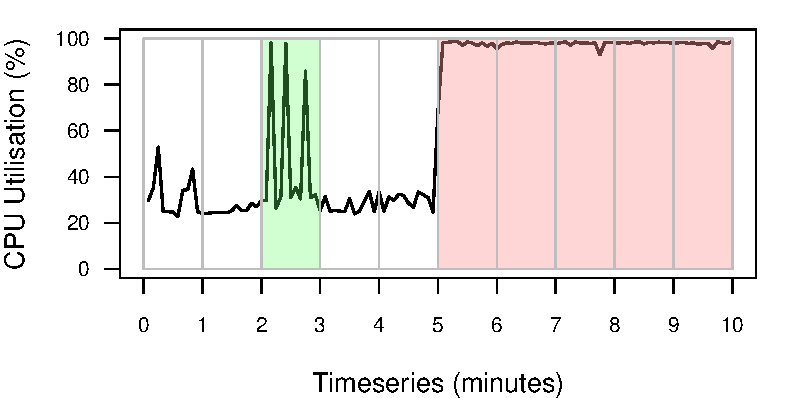
\epsfig{file = figures/approach_cpu_timeseries, width = 0.8\columnwidth}}
   \caption{Time series of CPU utilisation while running the Graph Analytics application. Pink coloured sections represent the utilisation during the \textit{anomaly-period} and green coloured section represents the utilisation with workload spikes during the \textit{normal-period}}
  \label{fig:cpu_timeseries}
  %\vspace{-0.1cm}
\end{figure}
%\vfill

% APPROACH CPU AVG, ENTROPY, SD 
%\vfill
\begin{figure}[!h]
  %\vspace{-0.2cm}
  \centering
   {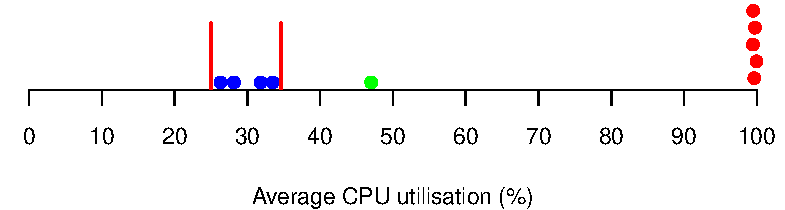
\epsfig{file = figures/approach_avg_dot, width = 0.8\columnwidth}}
     \hspace{0.9cm}
      {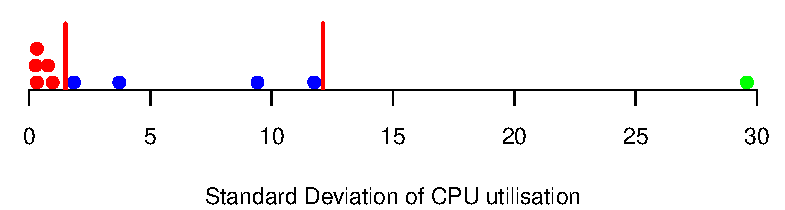
\epsfig{file = figures/approach_sd_dot, width = 0.8\columnwidth}}
        \hspace{0.9cm}
         {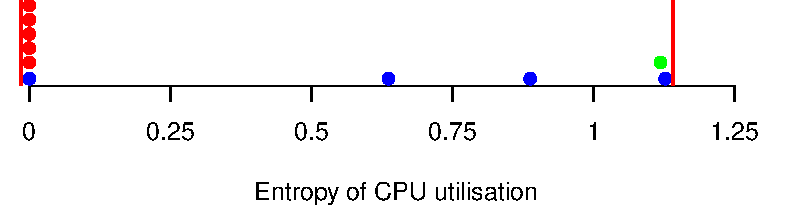
\epsfig{file = figures/approach_entropy_dot, width = 0.8\columnwidth}}
   \caption{Average, standard deviation, and entropy of CPU utilisation}
  \label{fig:avg_sd_entropy}
  %\vspace{-0.1cm}
\end{figure}
%\vfill

%\todo[author=DSN,inline]{It is not immediately clear what data processing techniques you are referring to here. Have you defined them or cited them earlier in the paper?}
%\todo[author=SB,inline]{Cited them now here, please check}
\textit{Window-based Time Series Analysis:} 
%Both the average and the entropy based time series analysis used in the Cloud anomaly detection systems such as~\cite{automated-detection:2016}, \cite{UBL:2012}, \cite{cloud-malware:2016}, \cite{EbAT:2010}, \cite{entorpy_based_detection_2:2014} are window-based, where the raw data are firstly distributed into a number of data bins with equal window size and secondly, the average or entropy of the data is calculated in each bin. These averages or entropies collected from the bins form the time series data to be used in the anomaly detection systems. 
%To produce the window-based time series data, we grouped the CPU utilisation data points into 10 data bins, each with a window size of 1 minute (the grey coloured partitions of the timeseries in Figure~\ref{fig:cpu_timeseries}) and then calculated three statistical measurements (average, standard deviation, and entropy) of the CPU utilisation in each bin. We selected the window size to be 1 minute as we experimentally found that anything shorter than this does not help in reducing the noise or spikes from the CPU utilisation and anything longer than this does not capture the short-term CPU utilisation behaviour.  
Anomaly detection systems which use linear classifiers, generally perform window-based time series analysis where the raw time series data are firstly distributed into a number of data bins with equal window size, and secondly, the average or entropy of the data is calculated in each bin. These averages or entropies collected from the bins form the time series data to be used in the anomaly detection systems.
To perform such an analysis, we grouped the CPU utilisation data points into 10 data bins, each with a window size of 1 minute (the grey coloured partitions of the time series in Figure~\ref{fig:cpu_timeseries}) and then calculated three statistical measurements (average, standard deviation, and entropy) of the CPU utilisation in each bin. We selected the window size to be 1 minute as we experimentally found that anything shorter than this does not help in reducing the noise from the CPU utilisation and anything longer than this does not capture the short-term CPU utilisation behaviour.  
%\textcolor{red} {We calculated the entropy using the equation ...}
%\textcolor{red}{Entropy [29] is calculated using the equation~\ref{eq1}. }%is a widely used measurement that captures the degree of dispersal or concentration of random variable distributions. 

For a discrete random variable $X$ with possible values $\big\{x_1,x_2...,x_n\big\}$ the entropy~\cite{entropy:2001} is calculated using Equation~\ref{entropy}. 
To prepare the data for the entropy calculation in each bin, we firstly normalise each of the raw data samples using Equation~\ref{normalisation} (normalised values are in the range $[0.0-1.0]$) and secondly, we decide to which amongst the following 10 smaller bins each normalised value belongs: 
$[0.0-0.1), [0.1-0.2), [0.2-0.3), [0.3-0.4), [0.4-0.5), [0.5-0.6), [0.6-0.7), [0.7-0.8), [0.8-0.9), [0.9-1.0]$. 
Finally, in each bin, we count the number of occurrences of the normalised values of the raw data samples in each smaller bin.
Thus, in Equation~\ref{entropy} we consider these numbers of occurrences as the values of the random variable $X$ in order to calculate the entropy.

We had 10 values (1 from each data bin) for each statistical measurement, which we present in Figure~\ref{fig:avg_sd_entropy} using 10 coloured dots along the x-axis. The 4 blue dots represent the measurements during the \textit{normal-period}, whereas the 5 red dots represent the measurements during the \textit{anomaly-period}. The green dot represents a measurement during the \textit{normal-period}, when the CPU encountered consecutive workload spikes (refers to the 3\textsuperscript{rd} minute in Figure~\ref{fig:cpu_timeseries}).

\begin{equation}
\label{entropy}
H(X) = -\sum\limits_{i=1}^n P(x_i)\log P(x_i)
\end{equation}
\begin{tabular}{l l}
     where &$P(x_i)$\;=\;probability mass function of $x_i$\\
                &$-logP(x_i)$\;=\;surprisal or self-information of $x_i$\\
\end{tabular}\\ 

\begin{equation}
\label{normalisation}
    X_{normalised} \quad = \quad   \frac{X - X_{min}}{X_{max} - X_{min}}
\end{equation}
\begin{tabular}{l l}
     where &$X_{normalised}$\;=\;normalised metric value\\
                &$X$\;=\;current metric value\\
                &$X_{min}$\;=\;minimum metric value in the raw data set \\
                &$X_{max}$\;=\;maximum metric value in the raw data set \\
\end{tabular}\\ \\ 

%In an ideal case of a linear classifier, we expected that the blue and the green dots are separable from the red dots by a hyperline. But, the measurements from Figure~\ref{fig:avg_sd_entropy} show different results. 
%From Figure~\ref{fig:avg_sd_entropy} we observe that, in the case of average, although the blue and the red dots are clearly separable by using a hyperline (the red line), the green dot falls on the wrong side of the hyperline. In case of standard deviation and entropy, we observe that even the blue and the red dots are not separable by any hyperline, instead the green dot becomes separable from both of them. 
%In an ideal case of an unsupervised learning or one class classifier, we expect that the blue and the green dots (normal behaviour data points) are clustered together in such a way that they are separable from the red dots (anomaly behaviour data points) by hyperplanes. But, the measurements from Figure~\ref{fig:avg_sd_entropy} show different results. 
%In case of unsupervised learning~\cite{automated-detection:2016}, \cite{UBL:2012} or one class classification~\cite{cloud-malware:2016} algorithms, the normal data points are clustered together and surrounded by hyperplanes and any data point outside those hyperplanes is considered as anomaly. For each statistical measurement, we tried to cluster the normal data points (blue and green dots) together and draw the hyperplanes (the red lines) surrounding them (see Figure~\ref{fig:avg_sd_entropy}). 
In the case of linear classifiers, the ``normal" data points are separated from the ``anomalous" data points by a hyperplane. 
%For each statistical measurement, we tried to cluster the normal data points (blue and green dots) together and draw the hyperplane (the red lines) to separate them from the anomalies (red dots) (see Figure~\ref{fig:avg_sd_entropy}). 
%For each statistical measurement, we considered that the anomalies (red dots) the genuine workload spikes (green dot) are appearing only during the testing or detection phase of the classifier and therefore, we tried to draw the hyperplane (the red lines) only considering the normal data points (blue dots) (see Figure~\ref{fig:avg_sd_entropy}). 
In this analysis, we consider that the anomalies (red dots) and the genuine workload spikes (green dot) are appearing only during the testing or detection phase of the classifier. Therefore, for each statistical measurement, we drew two hyperplanes (the red lines) by considering the minimum and the maximum values of the ``normal" data points (blue dots); Figure~\ref{fig:avg_sd_entropy} presents this. We expected that the green dot (workload spikes) resides within the hyperplanes as they belong to the \textit{normal-period} and the red dots (anomalies) are clearly separable by the hyperplanes as they belong to the \textit{anomaly-period} of the experiment. 
%red dots (anomalies) reside outside the hyperplanes as they belong to the \textit{anomaly-period} of the experiment.
%In case the genuine workload spikes are occurring during the training phase then using only approach (a) will suffice as in that case, the spike samples can be recorded as ``normal" by OCC algorithm. But, if the genuine workload spikes are not seen during the training phase and they are only appearing during the testing or the detection phase then we need to use both approach a and b. We consider the latter condition in our experimental evaluation.
%presents the classification amongst the blue, red, and green dots. But, we found that the green dot representing the genuine workload spikes resides outside the hyperplanes as it is far from the cluster of blue dots.
%From the figure we observe that, in case of average, the blue dots are closely clustered and the green dot representing the genuine workload spikes is far from this cluster and hence, it resides outside the hyperplane, indicating an anomaly.
%In case of standard deviation, although the blue dots are clustered together, the blue and the red dots are marginally separable by the left hyperplane, and importantly, the green dot moves very far from both the blue and the red dots.
%However, from the figure we observe that, in case of average, the blue dots are closely clustered and clearly separable from the red dots by the right hyperplane. However, the green dot representing the genuine workload spikes is far from the cluster of blue dots and hence, it resides outside the hyperplanes, indicating an anomaly.
%In case of standard deviation, although the blue dots are clustered together, the blue and the red dots are marginally separable by the left hyperplane, and importantly, the green dot moves very far from both the blue and the red dots.
From the figure we observe that, in the case of average, the blue dots are closely clustered and the red dots are clearly separable from them by the right hyperplane. However, the green dot representing the genuine workload spikes does not reside within the hyperplanes and indicates an anomaly.
In the case of standard deviation, although the blue dots are clustered together, the blue and the red dots are marginally separable by the left hyperplane, and importantly, the green dot does not reside within the hyperplanes and moves very far from both the blue and the red dots.
%outcome of which is discussed as follows: 
%they are separable from the red dots (anomaly behaviour data points) by hyperplanes. But, the measurements from Figure~\ref{fig:avg_sd_entropy} show different results. 
%From Figure~\ref{fig:avg_sd_entropy} we observe that, in case of average, although the blue and the red dots are clearly separable by using hyperplanes (the red lines), the green dot resides outside the hyperplanes as it is far from the cluster of blue dots.
%In case of standard deviation, we observe that the blue and the red dots are marginally separable by the hyperplanes and importantly, the green dot moves very far from both the blue and the red dots.
%In case of entropy, the blue dots are not clustered together and they are mixed with the red dots.
In the case of entropy, the blue and the red dots are not separable, although the green dot resides within the hyperplanes.
%even the blue and the red dots are not separable by any hyperplane.
From these observations we identify the following problems for Cloud anomaly detection systems:
\begin{enumerate}[{(1)}] 
%\item An average based linear classifier cannot differentiate between the ``normal" and the ``anomalous" VM resource utilisation behaviour if the VM encounters workload spikes. Specifically, they may wrongly identify the genuine Cloud workload spikes as anomalies and raise false positives.
\item An average based linear classifier may identify the genuine workload spikes as anomalies and raise false positives.
%\item Similar to average, a standard deviation based linear classifier may also raise false positives; additionally, it may even fail to identify anomalies and raise false negatives resulting in low detection accuracy.  
\item Similar to average, a standard deviation based linear classifier may also raise false positives. Additionally, it may even fail to differentiate between normal behaviour and anomalies, which may raise false negatives resulting in low classification accuracy.  
\item An entropy based linear classifier may not raise false positives; but, similar to standard deviation, it may result in low classification accuracy due to failure in differentiating between normal behaviour and anomalies.
%between the ``normal" and the ``anomalous" VM resource utilisation behaviour: in fact entropy based classifier fails even when the normal behaviour does not include workload spikes. Hence, they may fail to identify the anomalies and raise false negatives resulting into low detection accuracy. 
%\item Similar to average, standard deviation and entropy based linear classifiers also fail to differentiate between the ``normal" and the ``anomalous" VM resource utilisation behaviour: in fact entropy based classifier fails even when the normal behaviour does not include workload spikes. Hence, they may fail to identify the anomalies and raise false negatives resulting into low detection accuracy. 
%\begin{itemize}
%\item The average values cannot differentiate between the ``normal" and the ``anomalous" Cloud application behaviour if the normal behaviour encounters workload spikes. Specifically, any average based linear classifier may wrongly identify the genuine workload spikes as anomalies, which will increase the false alarms. 
%\item Similar to average, standard deviation and entropy fail to differentiate between the ``normal" and the ``anomalous" Cloud application behaviour: in fact they fail even when the normal behaviour does not have any workload spikes. Hence, any standard deviation and entropy based linear classifier may struggle to identify the anomalies due to security attack, which will reduce detection accuracy. 
%\item The average values cannot differentiate between the normal and the anomalous cloud application behaviour if the normal behaviour encounters instantaneous spikes. Specifically, if the spikes appear only during the testing or the detection phase and not during the training phase, then the classifier may wrongly identify the spikes as anomalies, which will increase the false alarms. 
%On one hand, if the spikes appear during the training period of an average based linear classifier, then the classifier may not successfully identify the anomalies, which will reduce the detection accuracy. On the other hand, if the spikes appear only during the testing or the detection phase, then the classifier may wrongly identify the spikes as anomalies, which will increase the false alarms. 
%\item Similar to average, standard deviation and entropy fail to differentiate between the normal and the anomalous cloud application behaviour, in fact they fail even when the normal behaviour does not have any instantaneous spikes. Hence, any  standard deviation and entropy based linear classifier may also suffer from accuracy and false alarm issues. 
\end{enumerate}
%\end{itemize}
%Researchers do not emphasise much on \textit{challenge 3}. They generally build the behavioural models with fixed training duration, which they usually decide based on offline experiments and they keep the duration constant throughout the intrusion detection process. Thus, they do not provide techniques to extract optimised duration for the training, which can be dynamically decided based on the online or real-time application resource utilisation pattern.
%\todo[author=DSN,inline]{This reads well but again, bares rather limited relevance to the Cloud. You could strengthen the motivation for this discussion by articulating that normal, non-anomalous spikes are a common behaviour in the Cloud. Ideally, you should back this claim up with citations.}
%\todo[author=SB,inline]{Please check the red texts in Introduction (in the discussion of challenges) where I have mentioned that spikes are more common in the Cloud with reference}
